\documentclass[12pt,letterpaper]{article}
\usepackage[frenchb]{babel}
\usepackage[margin=0.75in]{geometry}
\usepackage{hhline}
\usepackage{graphicx}
\graphicspath{ {images/} }

\title{Eclipse X - BMS}
\author{
	Daigneault-St-Arnaud, Christian, DAIC30099006
}
\newcommand{\cours}{ }
\newcommand{\prof}{ }


\begin{document}
	
	\begin{titlepage}
	\makeatletter
		\pagenumbering{gobble}
		\centering
		\vspace{5cm}
		{\Huge \@title}\\ 
		\vspace{5cm}
		{\large 
			Par \\
			\vspace{0.5cm}
			\@author \\
			\vspace{5cm}
			%\cours \\
			%\vspace{0.5cm}
			%\prof \\
			%\vspace{3.5cm}
			\@date \\
			\vspace{5cm}
			\'{E}COLE DE TECHNOLOGIE SUP\'{E}RIEURE \\
			UNIVERSIT\'{E} DU QUÉBEC
		}
		\newpage
	\end{titlepage}
	\tableofcontents
	\newpage
	\pagenumbering{arabic}
	\begin{normalsize}
		\section{Lecture de tension des modules}
			\subsection{Objectifs}
				objectif
			\subsection{Circuit analogique}
				Sch\'{e}ma du circuit : \\
				\begin{center}
					% Schema
					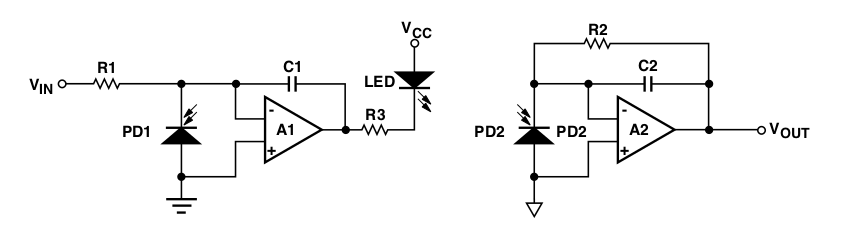
\includegraphics[scale=0.5]{Analog} \\ \vspace{1cm}
					%  BOM
					BOM \\ \vspace{0.25cm}
					\begin{tabular}{|c|c|c|}
						\hline
						Part number & Description & Prix (total)\\ \hhline{|=|=|=|}
						BU7421SG-TR & Op-amp (2x) & 2\$ \\ \hline
						LOC110STR & Optocoupleur lin\'{e}aire & 4.09\$ \\ \hline
						 \multicolumn{2}{|c|}{ }& 6.09\$ \\ \hline
						 \multicolumn{3}{r}{ } Prix de digikey pour 1 unit\'{e} \\
					\end{tabular}\\ \vspace{1cm}
					% Fin BOM
				
					% Avantage // Desavantage
					Analyse de la solution \\ \vspace{0.25cm}
					\begin{tabular}{|c|c|}
						\hline
						Avantage & D\'{e}savantage\\ \hhline{|=|=|}
						Peut de composantes & Pr\'{e}cision de +/- 1\% \\ \hline
						Robuste & L'optocoupleur lin\'{e}aire est gros (SOIC 8)\\ \hline
						 & Consomme beaucoup de courant (10mA max)\\ \hline
					\end{tabular} \\ \vspace{1cm}
					% Fin Avantage // Desavantage
				\end{center} 
				Conclusion
			\subsection{Circuit digital}
				\subsubsection{Protocole de communication}
					I2C\\
				\subsubsection{Lecture d'un voltage de reference}
				\subsubsection{Lecture du voltage de la cellule}
					MCP3221A5T => Non adressable
					ADC121C021CIMM/NOPB
				
	\end{normalsize}
\end{document}
\makeatother


